
\subsubsection{Ressourcen-Sharing}
Das Ziel\index{Ziele} des Ressource-Sharings in verteilten Systemen bezieht sich darauf, dass Ressourcen wie Hardware, Software und Daten zwischen verschiedenen Knoten und Anwendungen im System geteilt werden können. Durch das Teilen von Ressourcen können die Kosten und die Komplexität des Systems reduziert werden, während gleichzeitig die Effizienz und Skalierbarkeit erhöht werden können.

Ein aktuelles Beispiel für Ressourcen-Sharing in verteilten Systemen ist die Virtualisierungstechnologie, die es mehreren virtuellen Maschinen (VMs) oder Containern ermöglicht, auf einer einzigen physischen Hardware-Plattform zu laufen. Diese Technologie ermöglicht es, Ressourcen wie CPU, Speicher und Netzwerkbandbreite effektiv zwischen den verschiedenen VMs oder Containern zu teilen.

Für ein dezentrales Ressourcen-Sharing in verteilten Systemen ist die Blockchain-Technologie ein gutes Beispiel, die es in der einfachen Idee mehreren Knoten ermöglicht, gemeinsam auf eine dezentrale Datenbank zuzugreifen. Die Blockchain-Technologie ermöglicht es, Daten sicher und transparent zwischen den verschiedenen Knoten zu teilen und zu verwalten, ohne dass eine zentrale Autorität erforderlich ist. Dies kann die Effizienz und Skalierbarkeit des Systems erhöhen und die Kosten und Risiken durch Intermediäre reduzieren.

Ein weiteres aktuelles Thema ist die Cloud-Computing-Plattformen wie es beispielhaft in Amazon Web Services, Microsoft Azure oder Google Cloud bespielt wird. Unternehmen und Organisationen ermöglichen Ressourcen wie Rechenleistung, Speicher und Netzwerkbandbreite bei Bedarf dynamisch und flexibel zu teilen und zu nutzen. Durch das Teilen von Ressourcen können sie selbst - aber auch ihre Kunden insbesondere mittels Synergien - die Kosten reduzieren, die Effizienz erhöhen und schnell auf sich ändernde Anforderungen reagieren.

\subsubsection{Offenheit}
In dem Kontext von verteilten Systemen bezieht sich das Ziel der Offenheit oder engl. Openness darauf, dass ein System so konzipiert sein sollte, dass es leicht zugänglich und anpassbar für Benutzer und Entwickler ist. Ein offenes System ermöglicht es Benutzern und Entwicklern, auf seine Ressourcen und Funktionen über wohl-definierte Schnittstelen zuzugreifen.
\\\\
Ein offenes verteiltes System sollte auch in der Lage sein, mit anderen Systemen nahtlos zu interagieren, unabhängig davon, welche Plattformen oder Technologien sie verwenden. Dies ist besonders wichtig, da verteilte Systeme typischerweise aus einer Vielzahl von Hardware- und Softwarekomponenten bestehen können, die von verschiedenen Anbietern stammen und auf unterschiedlichen Plattformen laufen. Ein offenes System kann die Interoperabilität und Zusammenarbeit zwischen diesen verschiedenen Komponenten verbessern.
\\\\
Ein weiteres Ziel der Offenheit in verteilten Systemen ist die Förderung von Innovation und Wettbewerb. Durch die Bereitstellung offener Standards und Schnittstellen können Benutzer und Entwickler neue Anwendungen und Dienste erstellen, die auf verschiedenen Systemen und Plattformen laufen können. Dies kann zu einem größeren Angebot an Produkten und Dienstleistungen führen, die den Bedürfnissen der Benutzer besser entsprechen und gleichzeitig die Kosten senken und die Flexibilität erhöhen.
\\\\
Durch die Schaffung offener Standards und Schnittstellen kann auch die Zusammenarbeit und Interoperabilität zwischen verschiedenen Systemen und Plattformen verbessert werden. Es gibt einige Beispiele dafür, wie Openness in verteilten Systemen eingesetzt werden kann. Hier sind einige Beispiele:
\begin{itemize}
\item \textbf{Offene Standards} für die Kommunikation: Die Verwendung offener Standards wie HTTP, XML oder JSON ermöglicht es verschiedenen Systemen, miteinander zu kommunizieren, unabhängig von der Plattform oder Technologie, auf der sie laufen. Dies fördert die Interoperabilität zwischen verschiedenen Systemen und erleichtert die Integration von Drittanbieterkomponenten in verteilten Systemen.
\item \textbf{Open-Source-Software}: Die Verwendung von Open-Source-Software in verteilten Systemen ermöglicht es den Entwicklern, den Quellcode anzupassen und zu erweitern, um die Anforderungen des Systems zu erfüllen. Dies fördert die Flexibilität und ermöglicht es, spezielle Funktionen zu implementieren, die möglicherweise nicht in proprietären Lösungen verfügbar sind.
\item \textbf{Wohl-definierte APIs}: Die Bereitstellung wohl-definierter APIs (Application Programming Interfaces) ermöglicht es Drittanbietern, auf die Funktionen und Dienste eines verteilten Systems zuzugreifen und diese zu erweitern. Dies fördert die Flexibilität und ermöglicht es, die Funktionen des verteilten Systems an die Bedürfnisse der Benutzer anzupassen.
\item \textbf{Offene Datenformate}: Die Verwendung offener Datenformate wie CSV oder RDF ermöglicht es verschiedenen Systemen, Daten auszutauschen und zu verarbeiten, unabhängig von der Plattform oder Technologie, auf der sie laufen. Dies fördert die Interoperabilität und erleichtert den Austausch von Daten zwischen verschiedenen Systemen.
\end{itemize}
In der Lehre ist dieses Ziel im Vergleich schwer zu vermitteln, da die Konsequenzen bei nicht Erreichung erst zu einem späteren Zeitpunkt in einem Application-Life-Cycle sichtbar werden. Die Wichtigkeit kann aber nicht überbetont werden. 

\subsubsection{Skalierbarkeit}
Das Ziel der Skalierung oder engl. Scalability im Kontext von verteilten Systemen bezieht sich darauf, dass ein System in der Lage sein sollte, mit wachsenden Anforderungen und steigenden Benutzerzahlen umzugehen, ohne dabei an Leistung oder Stabilität zu verlieren. Es geht also darum, sicherzustellen, dass ein verteiltes System in der Lage ist, seine Funktionalität und Leistungsfähigkeit bei Bedarf zu erhöhen.

Skalierbarkeit ist ein wichtiges Ziel für verteilte Systeme, da diese Systeme typischerweise sehr große und komplexe Aufgaben bewältigen müssen, die eine enorme Rechenleistung und Ressourcen erfordern können. Wenn ein System nicht skalierbar ist, kann es schnell an seine Grenzen stoßen und die Leistung und Verfügbarkeit des Systems beeinträchtigen. Eine gute Skalierbarkeit ist daher entscheidend für die erfolgreiche Umsetzung von Verteilten Systemen.

Es gibt verschiedene Ansätze, um die Skalierbarkeit von verteilten Systemen zu verbessern. Einer dieser Ansätze ist die Verwendung von skalierbaren Architekturen, die aus Modulen bestehen, die horizontal oder vertikal skalieren können. 

\begin{itemize}
\item \textbf{Vertikale Skalierung\index{Vertikale Skalierung}} bezieht sich auf das Hinzufügen weiterer Ressourcen (z.B. CPU, RAM, Speicher) zu einem einzelnen Server, um dessen Leistungsfähigkeit zu erhöhen. Mit anderen Worten, das System wird durch eine Erhöhung der Kapazität eines einzelnen Servers verbessert. Beispielsweise kann ein System mit vertikaler Skalierung mit einer leistungsstärkeren CPU oder einer höheren RAM-Kapazität ausgestattet werden, um eine höhere Arbeitslast zu bewältigen. Diese Art der Skalierung ist besonders nützlich, wenn das System mehr Rechenleistung benötigt, um komplexe Operationen auszuführen oder große Datenmengen zu verarbeiten. Zu bemerken ist vielleicht, dass die vertikale Skalierung nicht die Umsetzung mit einem System verlangt, sondern die Skalierung in den festen Größen (Anzahl der Server) der Systemarchitektur. 

\item \textbf{Horizontale Skalierung\index{Horizontale Skalierung}} dagegen bezieht sich auf das Hinzufügen weiterer Ressourcen (z.B. Server) zu einem System, um die Leistungsfähigkeit zu verbessern. Mit anderen Worten, mehrere Knoten werden hinzugefügt, um die Arbeitslast auf mehrere Server aufzuteilen. Beispielsweise kann ein System mit horizontaler Skalierung so konfiguriert werden, dass es Anfragen auf mehrere Server aufteilt, wodurch eine höhere Anzahl von Anfragen gleichzeitig verarbeitet werden kann. Diese Art der Skalierung ist besonders nützlich, wenn das System auf eine hohe Anzahl von Anfragen oder eine erhöhte Datenmenge reagieren muss.
\end{itemize}

Einfach gesprochen sollte man sich merken, das Horizontale Skalierung  eine höhere Ausfallsicherheit und verbesserte Leistung bei hohen Anfragemengen ermöglicht, es jedoch mehr Koordination zwischen den verschiedenen Servern erfordert. Vertikale Skalierung hingegen ist einfacher zu verwalten, aber die Kapazität eines einzelnen Servers ist begrenzt und kann irgendwann erschöpft sein.
\\\\
Ein weiterer Ansatz besteht darin, die Lastverteilung zu optimieren, um sicherzustellen, dass die Ressourcen des Systems effizient genutzt werden. Hierbei können verschiedene Technologien wie Load-Balancer oder verteilte Datenbanken zum Einsatz kommen. Um den verschiedenen Zielen der Skalierung gerecht zu werden, unterscheidet~\cite{tanenbaum2017distributed} in drei Unterzielen:
\begin{itemize}
\item \textbf{Räumliche Skalierbarkeit}: Das Ziel der räumlichen Skalierung in verteilten Systemen bezieht sich darauf, dass das System effektiv und effizient auf verschiedene geografische Standorte oder Regionen ausgedehnt werden kann. Dies bedeutet, dass das System in der Lage sein muss, mit unterschiedlichen Netzwerkbedingungen, geografischen Entfernungen und Latenzzeiten umzugehen, um eine reibungslose und effektive Kommunikation zwischen den verschiedenen Standorten zu gewährleisten.

Ein aktuelles Beispiel für die räumliche Skalierung in verteilten Systemen ist die Cloud-Computing-Plattform von Amazon Web Services (AWS). AWS ist in der Lage, Anwendungen und Services auf verschiedene geografische Regionen auszudehnen, um die Bedürfnisse von Kunden auf der ganzen Welt zu erfüllen. AWS bietet eine Vielzahl von Funktionen und Tools, die es Entwicklern und Administratoren ermöglichen, Anwendungen und Services in verschiedenen Regionen und Zonen zu konfigurieren und zu skalieren, um eine optimale Leistung und Verfügbarkeit zu gewährleisten. Dazu gehören Funktionen wie automatische Lastverteilung, Regionen und Zonen-Management, Netzwerk-Isolation und Latenzoptimierung. Man muss aber auch in diesem Zusammenhang beachten, das eine Abhängigkeit zu Anbietern solcher Infrastrukturkomponenten auch eine durchaus relevante Gefahr für den Anwendungsfall sein kann.

Ein weiteres Beispiel für die räumliche Skalierung sind die Content-Delivery-Netzwerke (CDN), die es Unternehmen und Organisationen ermöglichen, Inhalte und Anwendungen effektiv auf globaler Ebene bereitzustellen. Ein Beispiel für ein CDN ist Akamai, das ein Netzwerk von Servern auf der ganzen Welt betreibt, um eine schnelle und effektive Bereitstellung von Inhalten und Anwendungen zu gewährleisten. Akamai und andere CDN-Anbieter verwenden angepasste Algorithmen und Tools, um Inhalte und Anwendungen auf den am besten geeigneten Servern und Standorten zu verteilen, um eine optimale Leistung und Verfügbarkeit zu gewährleisten.

\item \textbf{Funktionale Skalierbarkeit}: Dieses Unterziel bezieht sich auf die Fähigkeit eines verteilten Systems, die Anzahl der unterstützten Funktionen und Dienste zu erhöhen, ohne dass dies zu einer Abnahme der Leistung oder Stabilität führt. Eine funktional skalierbare Architektur ermöglicht es einem verteilten System, neue Dienste oder Funktionen hinzuzufügen, um sich an sich ändernde Geschäftsanforderungen oder Benutzerbedürfnisse anzupassen. Häufig ist diese Skalierbarkeit auch abhängig von der Problemgröße. Die Problemgröße bezieht sich auf die Menge an Daten, die in einem bestimmten Problem oder einer bestimmten Aufgabe verarbeitet werden müssen. Die Größe des Problems hängt von verschiedenen Faktoren ab, wie der Anzahl der Eingabevariablen, der Größe der Eingabedaten, der Anzahl der Ausgabevariablen oder der Komplexität des Algorithmus, der zur Lösung des Problems verwendet wird. Die Problemgröße kann sich auf verschiedene Arten auswirken, wie beispielsweise auf die Zeit, die benötigt wird, um das Problem zu lösen, oder auf den benötigten Speicherplatz, um die Daten zu speichern. In der Regel gilt, dass größere Probleme mehr Rechenleistung und Speicherplatz erfordern und daher mehr Zeit benötigen, um gelöst zu werden, wobei Teile der Arbeit in einem verteilten System parallelisiert werden können. Können Arbeiten parallelisiert werden, kann man es sich wie eine Stapelverarbeitung vorstellen, wo ein Stapel von Anträgen nicht von einer Person bearbeitet wird, sondern von einer Vielzahl von Personen. Der Stapel der Anträge dient als Sammelpunkt der Aufgaben und es braucht einen adäquaten Mechanismus um die Anträge an die bearbeitenden Personen zu verteilen. Hier gibt es verschiedene Gesetzmässigkeiten zu beachten, wie Little's Law~\cite{little1961proof}:

\textbf{Little's Law\index{Little's Law}} ist ein Gesetz der Warteschlangentheorie, das besagt, dass die durchschnittliche Anzahl von Kunden in einem System gleich der Produktivität des Systems multipliziert mit der durchschnittlichen Zeit, die ein Kunde im System verbringt, ist. Im Kontext von verteilten Systemen bedeutet dies, dass die Problemgröße eines verteilten Systems direkt mit der Anzahl der in diesem System aktiven Prozesse oder Anfragen zusammenhängt.

Insbesondere besagt Little's Law, dass die durchschnittliche Anzahl von Kunden in einem System, die in einer Warteschlange auf eine Antwort warten, direkt proportional zur durchschnittlichen Zeit ist, die ein Kunde im System verbringt, und zur durchschnittlichen Ankunftsrate der Kunden im System. Wenn wir dies auf ein verteiltes System anwenden, können wir sagen, dass die Anzahl der in einem verteilten System aktiven Prozesse oder Anfragen direkt proportional zur Größe des Systems und zur Rate ist, mit der neue Prozesse oder Anfragen im System ankommen.

Daher kann die Anwendung von Little's Law auf verteilte Systeme dazu beitragen, die Größe des Systems zu optimieren, um eine effiziente und zuverlässige Leistung zu gewährleisten. Eine Erhöhung der Anzahl der Prozesse oder Anfragen kann dazu führen, dass die Antwortzeiten steigen und die Leistung des Systems beeinträchtigt wird. Daher kann die Optimierung der Größe des Systems und der Ankunftsrate von Prozessen oder Anfragen dazu beitragen, die Leistung des verteilten Systems zu verbessern und eine optimale Problemgröße zu erreichen.

Hierdurch lassen sich auch erste Annahmen über die Einschränkungen der Skalierung machen. Die Skalierbarkeit eines Systems ist begrenzt, wenn die Ankunftsrate von Kunden oder Prozessen zu hoch wird und das System nicht in der Lage ist, die Anfragen innerhalb einer akzeptablen Zeit zu verarbeiten. Eine zu hohe Ankunftsrate kann zu Engpässen, Überlastungen und unakzeptablen Antwortzeiten führen, was sich negativ auf die Leistung des Systems auswirkt. 

Auch eine andere Grenze wird bei der Betrachtung der Skalierung deutlich, welche auftritt, wenn man das Verteilte System als Warteschlange mit vielen Bedienern betrachtet. Die Aufgaben müssen in einem Maße parallelisierbar sein, dass jeder Bediener auch ausreichend zu tuen bekommt und die Aufteilung ist ein zusätzlicher Aufwand, der berücksichtigt werden muss. Dieses muss bei der Konzeptionierung eines verteilten Systems berücksichtigt werden, und kann mit dem Gustafsons Gesetz\index{Gustafson}~\cite{gustafson1988reevaluating} diskutiert werden: 

Das Gesetz besagt, dass mit einer Erhöhung der Anzahl von Prozessoren die Größe des Problems, das gelöst werden kann, erhöht werden kann, während die Zeit, die zur Lösung des Problems benötigt wird, relativ stabil bleibt. Das bedeutet, dass das System durch Hinzufügen von Prozessoren oder Knoten skaliert werden kann, um größere Probleme effizienter zu lösen.

Ein Beispiel für die Anwendung von Gustafsons Gesetz auf die Konzeptionierung eines verteilten Systems könnte folgendermaßen aussehen: Angenommen, ein verteiltes System soll eine große Menge von Daten verarbeiten und analysieren, um ein bestimmtes Ergebnis zu liefern. Die Datenmenge wird als 100 GB angenommen, und das System soll innerhalb von 10 Minuten eine Analyse durchführen und das Ergebnis liefern.

Die Entwickler des verteilten Systems müssen nun entscheiden, wie viele Prozessoren oder Knoten sie verwenden möchten, um das Ziel der Analyse innerhalb der vorgegebenen Zeit zu erreichen. Wenn das System auf einem einzelnen Knoten ausgeführt wird, kann es möglicherweise die Datenmenge nicht innerhalb von 10 Minuten verarbeiten. Daher ist es erforderlich, das System horizontal zu skalieren, indem mehr Knoten hinzugefügt werden.

Angenommen, das verteilte System besteht aus 4 Knoten, und jeder Knoten kann 25 GB Daten in 2,5 Minuten analysieren. Durch Hinzufügen von Knoten wird die Größe des Problems erhöht, das System kann jedoch immer noch das Ziel der Analyse innerhalb der vorgegebenen 10 Minuten erreichen.

Diese Annahmen treffen aber nur zu, wenn die eingesetzten Algorithmen diese Skalierung durch ausreichende Parallelisierung stützen. Das Amdahlsche Gesetz\index{Amdahl}~\cite{amdahl1967validity} besagt, dass die Leistungssteigerung durch die Parallelisierung eines Systems begrenzt ist durch den Anteil der Berechnungen, der nicht parallelisiert werden kann. Das bedeutet, dass bei der Optimierung der Leistung eines Systems durch Parallelisierung die nicht-parallelisierbaren Anteile minimiert werden sollten, um eine optimale Leistungssteigerung zu erreichen. Ein Beispiel soll dies verdeutlichen:

Angenommen, es existiert eine Aufgabe, die aus zwei Teilaufgaben besteht: Eine Teilaufgabe ist zu 95\% nicht parallelisierbar in einer Schleife. Wie viel schneller wird das System im Vergleich zur Ausführung auf einem einzelnen Prozessor sein, wenn es auf 8 Prozessoren skaliert?

Um dies zu berechnen, können wir das Amdahlsche Gesetz anwenden. Laut dem Gesetz ist die maximale Beschleunigung, die wir durch Parallelisierung erzielen können, durch den Anteil der sequenziell ausgeführten Berechnungen begrenzt. 
Die maximale Beschleunigung, die wir erreichen können, wird als Speedup\index{Speedup} bezeichnet. Der Speedup kann als Maß für die Effizienz der Parallelisierung verwendet werden und wird wie folgt berechnet:

\begin{equation*}
Speedup = \frac{T_1}{T_p}
\end{equation*}

Dabei steht $T_1$ für die Ausführungszeit der Aufgabe auf einem einzelnen Prozessor (ohne Parallesierung) und $T_p$ für die Ausführungszeit der Aufgabe auf einem parallelen System mit $p$ Prozessoren (mit Parallesierung). Ein Speedup von $s$ bedeutet, dass das System auf $s$-fache Geschwindigkeit beschleunigt wurde im Vergleich zur Ausführung auf einem einzelnen Prozessor. Ein idealer Speedup von $p$ würde bedeuten, dass die Aufgabe auf $p$ Prozessoren $p$-mal schneller ausgeführt wird als auf einem einzelnen Prozessor. $P$ ist der parallesierbare Anteil, $N$ sind die Anzahl der Prozessoren:

\begin{align*}
Speedup &= \frac{1}{(1 - P) + (1 - P)/N} \
&= \frac{1}{0.05 + (1 - 0.05)/8} \
&= 5.9
\end{align*}

Das bedeutet, dass das System, welches die Aufgabe auf 8 Prozessoren ausführt, nicht schneller arbeiten wird als 6 Prozessoren. Die parallele Ausführung der Teilaufgaben hat keine Auswirkungen auf die Gesamtzeit, da es keinen sequenziell auszuführenden Anteil gibt, der durch Parallelisierung beschleunigt werden kann.

In diesem Beispiel zeigt das Amdahlsche Gesetz, dass die parallele Ausführung der Teilaufgaben in diesem System keinen Leistungsvorteil bietet, da der sequenziell auszuführende Anteil bestimmend ist. Dieses muss immer als Grundlage für das Gustafsons Gesetz verstanden werden.

\begin{figure}[!h]
\centering
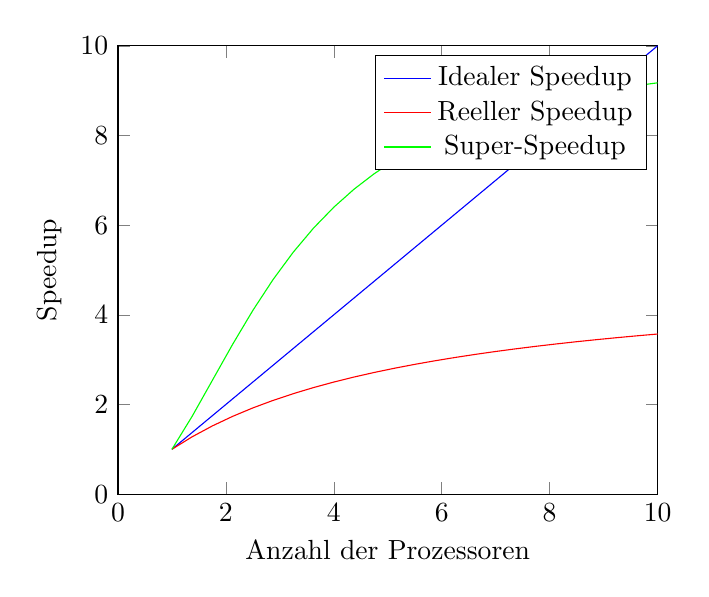
\begin{tikzpicture}
\begin{axis}[
  xlabel={Anzahl der Prozessoren},
  ylabel={Speedup},
  xmin=0, xmax=10,
  ymin=0, ymax=10,
  legend entries={Idealer Speedup, Reeller Speedup, Super-Speedup}
]
% Idealer Speedup
\addplot[blue, domain=1:10] {x};

% Reeller Speedup
\addplot[red, domain=1:10] {x/(1 + (x-1) * 0.2)};

% Superspeedup
\addplot[green, domain=1:10] {x^3/(x + (x^3-x) * 0.1)};
\end{axis}
\end{tikzpicture}
\caption{Speedup}
\label{fig:speedup}
\end{figure}

In der Grafik~\ref{fig:speedup} repräsentiert die blaue Linie den idealen Speedup, bei dem die Leistung linear mit der Anzahl der Prozessoren zunimmt. Die rote Linie zeigt den realen Speedup, der in der Regel geringer als der ideale Speedup ist. Die letzte Kurve beschreibt den Super-Speedup.
In verteilten Systemen kann ein sogenannter \enquote{Superspeedup} erreicht werden, wenn die Berechnungen und Prozesse über mehrere Rechner oder Knoten verteilt werden, was zu einer signifikanten Verbesserung der Leistung führt und zusätzlich Caching Mechanismen genutzt werden, die auf einer einzelnen CPU nicht möglich wären.\\
\\
Wie auch immer, zu Beginn der Entwicklung eines Verteilten Systems steht häufig noch nicht fest, in wie weit das System langfristig skalieren soll, daher sind auch schon kleine Systeme mit ausreichend Skalierungsmöglichkeiten zu designen und damit auch mit einem hohen Maß an möglicher Parallelität. Dies kann bereits in kleinen Entscheidungen bereits einen großen Unterschied machen, wie beispielhaft in der Auswahl der Sortieralgorithmen.

Hier sollen beispielhaft zunächst zwei Gründe aufgeführt werden, warum die Auswahl von Mergesort sich in einer generischen Diskussion besser eignet, als die Wahl von Quicksort. Diese Diskussion soll einzig die Detailtiefe der Überlegungen andeuten. 

Zunächst steht hier der Kommunikationsaufwand: Bei Quicksort müssen die Teillisten für jeden rekursiven Aufruf aufgeteilt und zwischen verschiedenen Knoten im verteilten System ausgetauscht werden. Dies erzeugt einen hohen Kommunikationsaufwand zwischen den Knoten, der die Gesamtleistung des verteilten Systems beeinträchtigen kann. Im Gegensatz dazu kann Mergesort leichter parallelisiert werden, indem die sortierten Teillisten fusioniert werden, um die endgültige sortierte Liste zu erstellen. Hierdurch wird der Kommunikationsaufwand reduziert.

Weiter existiert das Risiko des schlecht gewählten Pivot-Elements:
Wenn das Pivot-Element nicht sorgfältig ausgewählt wird, kann dies zu einer ungleichmäßigen Verteilung der Arbeit führen. Ein schlecht gewähltes Pivot-Element kann dazu führen, dass eine Teilliste ungewöhnlich groß wird und mehr Zeit benötigt, um sortiert zu werden als die anderen Teillisten. Infolgedessen können einige Knoten im verteilten System stark belastet werden, während andere Knoten inaktiv bleiben, was die Gesamtleistung des Systems beeinträchtigt.

Dies macht deutlich, dass bei der Konzeptionierung eines skalierenden Systems, nicht nur Anforderungen an das Problemverständnis gestellt werden, sondern auch eine breite Expertise. Diese umfasst eine tiefe Kenntnis über die möglichen Lösungskorridore  und ihrer bestimmenden Eigenschaften. 

Am Ende sollte noch eine weitere Gesetzmäßigkeit  für die Skalierung verinnerlicht werden. Brooks\index{Brook} sagt aus, dass die Komplexität eines Systems nicht durch Hinzufügen von Ressourcen reduziert werden kann. Mit anderen Worten, wenn ein System zu komplex ist, wird es nicht einfacher, nur weil man mehr Ressourcen hinzufügt. Diese Gesetzmäßigkeit wird aber viel zu oft in der Praxis ignoriert. 

\item \textbf{Verwaltungs- oder Administrative-Skalierbarkeit}: Verwaltungs- oder administrative Skalierbarkeit bezieht sich auf die Fähigkeit eines verteilten Systems, effektiv und effizient von Administratoren oder Betreibern verwaltet und überwacht zu werden, unabhängig von der Größe oder Komplexität des Systems. Dies ist besonders wichtig, da verteilte Systeme in der Regel aus einer Vielzahl von Komponenten und Knoten bestehen, die auf verschiedenen Hardware- und Software-Plattformen laufen und in verschiedenen Netzwerken miteinander kommunizieren.

Ein wichtiges Ziel der Verwaltungs- oder Administrative-Skalierbarkeit ist es, eine konsistente und zuverlässige Überwachung, Konfiguration und Verwaltung von verteilten Systemen zu ermöglichen, unabhängig von der Größe oder Komplexität des Systems. Dies kann durch die Verwendung von automatisierten Tools und Prozessen erreicht werden, die es Administratoren ermöglichen, das System zentralisiert und effektiv zu überwachen und zu verwalten.

Ein aktuelles Beispiel für ein verteiltes System mit hoher Verwaltungs- oder administrative Skalierbarkeit ist Kubernetes, eine Open-Source-Plattform zur Verwaltung von containerisierten Anwendungen. Kubernetes bietet eine Vielzahl von Funktionen und Tools, die es Administratoren ermöglichen, containerisierte Anwendungen effektiv zu verwalten, unabhängig von der Größe oder Komplexität des Systems. Dazu gehören Funktionen wie automatische Skalierung, Lastenausgleich, Fehlerbehebung, Überwachung und Protokollierung.

Ein weiteres Beispiel ist Apache ZooKeeper, eine Open-Source-Software zur Koordination von verteilten Anwendungen. ZooKeeper bietet Funktionen wie Synchronisierung, Konfiguration, Überwachung und Benachrichtigung, die es Administratoren ermöglichen, komplexe verteilte Anwendungen effektiv und effizient zu verwalten und zu überwachen.
\end{itemize}

\subsubsection{Verteilungstransparenz}

Das Ziel der Verteilungstransparenz in verteilten Systemen bezieht sich darauf, dass Benutzer und Anwendungen nicht bewusst sein sollten, dass sie auf ein verteiltes System zugreifen, d.h. das verteilte System sollte für sie transparent sein. Dies bedeutet, dass der Benutzer oder die Anwendung keine Kenntnis von der Anzahl der Knoten im System, ihrer physischen Speicherorte, der Kommunikationsmechanismen oder der Art und Weise haben sollte, wie die Daten im System verteilt sind oder wie die Auslastung des Systems ist.
\\\\
Die Verteilungstransparenz ist in der Tat ein schwieriges Ziel, da es viele widersprüchliche Anforderungen gibt, die erfüllt werden müssen. Einerseits muss das verteilte System in der Lage sein, effektiv mit verschiedenen Komponenten und Knoten zu kommunizieren und Ressourcen zu teilen, andererseits darf dies jedoch nicht zu einer Beeinträchtigung der Leistung oder Verfügbarkeit des Systems führen. Darüber hinaus muss das verteilte System sicher und zuverlässig sein, um sicherzustellen, dass Daten und Informationen nicht kompromittiert werden oder verloren gehen.

Es ist daher richtig, dass die Verteilungstransparenz nie zu 100\% erreicht werden kann, da es immer einige Aspekte gibt, die für den Benutzer oder die Anwendung nicht transparent sind. Zum Beispiel kann die Latenzzeit bei der Übertragung von Daten zwischen verschiedenen Knoten im System nicht vollständig beseitigt werden, was zu einer gewissen Verzögerung führt.  Selbst Licht, so müssen wir feststellen, ist für die Kommunikation nicht selten zu langsam. Ebenso kann es aufgrund der Verteilung der Daten im System nicht immer möglich sein, einen vollständigen Überblick über alle Daten im System zu haben.
\\\\
Trotz dieser Herausforderungen ist die Verteilungstransparenz ein wichtiges Ziel in verteilten Systemen, da sie die Effizienz und Skalierbarkeit des Systems erhöht und die Komplexität und die Kosten reduziert. Obwohl die Verteilungstransparenz nie vollständig erreicht werden kann, gibt es verschiedene Technologien und Ansätze, die genutzt werden können, um sie zu verbessern, wie zum Beispiel Load Balancing, Replikation, Caching und Datenpartitionierung.

Da es ein schwieriges Feld ist dieses Ziel zu erreichen, greift der informierte Informatiker auch in diesem Fall nicht ungern wieder auf die Teile-und-herrsche Methode zurück, die es erlaubt die einzelnen Anforderungsaspekte besser zu verstehen und geeignet, des gewünschten Grades nach, umzusetzen:
\begin{itemize}
\item  \textbf{Zugriffstransparenz}: Sie ist eine Art der Transparenz in verteilten Systemen, die darauf abzielt, dem Benutzer den Zugriff auf Ressourcen im Netzwerk so einfach wie möglich zu machen. Der Benutzer sollte in der Lage sein, auf Ressourcen zuzugreifen, ohne sich darüber Gedanken machen zu müssen, wo sich die Ressourcen befinden oder wie sie zugänglich gemacht werden können.

Ein Beispiel für Zugriffstransparenz ist die Verwendung von Dienstvermittlung. Hierbei wird ein zentraler Dienst eingerichtet, der Benutzern dabei hilft, auf Ressourcen im Netzwerk zuzugreifen, ohne dass sie sich über den genauen Standort oder die Eigenschaften der Ressourcen Gedanken machen müssen. Der Dienst kann beispielsweise die Namen von Diensten und Ressourcen im Netzwerk bereitstellen und den Benutzer auf die entsprechenden Ressourcen weiterleiten.

Ein Weg für die Erreichung der Zugriffstransparenz ist die Verwendung von Adressauflösung. Hierbei wird eine Adresse verwendet, um auf eine Ressource im Netzwerk zuzugreifen, ohne dass der Benutzer sich über den genauen Standort der Ressource Gedanken machen muss. Die Adressauflösung kann automatisch erfolgen, indem beispielsweise ein Domain Name System (DNS) verwendet wird.

Netzwerkprotokolle sind ebenfalls ein wichtiger Bestandteil der Zugriffstransparenz. Durch die Verwendung von Netzwerkprotokollen und damit verbundenen Schichtenmodellen können Benutzer auf Ressourcen im Netzwerk zugreifen, ohne sich Gedanken darüber machen zu müssen, wie die Kommunikation zwischen den Komponenten erfolgt oder wie Daten über das Netzwerk übertragen werden.

\item \textbf{Lokalitäts-Transparenz}: Diese Transparenz zielt darauf ab, dem Benutzer die Komplexität des Systems zu verbergen, indem ihm das \enquote{Gefühl} vermittelt wird, dass Ressourcen lokal verfügbar sind, auch wenn sie sich in Wirklichkeit an einem entfernten Ort befinden. Mit anderen Worten, Lokalitäts-Transparenz bedeutet, dass der Benutzer nicht wissen oder sich darum kümmern muss, wo sich eine bestimmte Ressource im Netzwerk befindet oder wie sie zugänglich gemacht wird.

Ein Beispiel für Lokalitäts-Transparenz ist die Verwendung von virtuellen Ressourcen. Durch die Erstellung von virtuellen Ressourcen, wie virtuellen Maschinen oder virtuellen Festplatten, können Ressourcen im Netzwerk bereitgestellt werden, ohne dass der Benutzer sich Gedanken darüber machen muss, wo sich die physischen Ressourcen befinden.

Ein weiteres Beispiel für Lokalitäts-Transparenz ist die Verwendung von Dateisystemen. Durch die Verwendung von verteilten Dateisystemen kann der Benutzer auf Dateien zugreifen, ohne sich Gedanken darüber machen zu müssen, wo sich die Dateien im Netzwerk befinden. Das verteilte Dateisystem sorgt dafür, dass der Benutzer auf die Dateien zugreifen kann, als ob sie sich lokal auf seinem Gerät befinden.

Lokalitäts-Transparenz kann auch durch die Verwendung von Replikation erreicht werden. Durch die Replikation von Ressourcen auf verschiedene Knoten im Netzwerk kann der Benutzer auf die Ressourcen zugreifen, ohne sich Gedanken darüber machen zu müssen, wo sich die Ressourcen befinden oder welche Knoten verfügbar sind. 

\item \textbf{Migrationstransparenz}: Die Transparenz ermöglicht den Benutzern, von einem Ort oder Gerät zu einem anderen zu wechseln, ohne dabei ihre Sitzung oder den Zugriff auf ihre Ressourcen zu verlieren. Mit anderen Worten, die Migrationstransparenz ermöglicht es dem Benutzer, nahtlos zwischen verschiedenen Geräten oder Standorten zu wechseln, ohne dass er seine Arbeit unterbrechen oder sich neu anmelden muss.

Ein Beispiel für Migrationstransparenz ist die Verwendung von Virtualisierungstechnologien. Durch ihre Verwendung können Benutzer ihre Arbeitsumgebung in einer virtuellen Maschine speichern und auf verschiedenen Geräten ausführen, ohne ihre Sitzung oder den Zugriff auf ihre Ressourcen zu verlieren. Wenn der Benutzer beispielsweise von einem Laptop zu einem Desktop-Computer wechselt, kann er einfach die virtuelle Maschine auf dem Desktop öffnen und seine Arbeit fortsetzen, ohne dass er seine Sitzung unterbrechen oder sich erneut anmelden muss.

Auch die die Verwendung von Cloud-basierten Diensten ist ein gutes Beispiel für Migrationstransparenz. Durch die Verwendung  können Benutzer auf ihre Ressourcen zugreifen, unabhängig von ihrem Standort oder dem Gerät, das sie verwenden. Wenn der Benutzer beispielsweise von einem mobilen Gerät auf einen Desktop-Computer wechselt, kann er einfach auf sie zugreifen und seine Arbeit fortsetzen, ohne seine Sitzung unterbrechen zu müssen.

Die Migrationstransparenz wird oft durch Mechanismen wie Sitzungs- und Zustandssynchronisierung, Lastverteilung und automatische Skalierung erreicht. Sitzungs- und Zustandssynchronisierung ermöglicht es Benutzern, ihre Sitzungen und Zustände zwischen verschiedenen Geräten oder Standorten zu synchronisieren. Lastverteilung und automatische Skalierung sorgen dafür, dass die Ressourcen im System je nach Bedarf automatisch skaliert und verteilt werden, um eine unterbrechungsfreie Benutzererfahrung zu gewährleisten.

\item \textbf{Replikationstransparenz}:  Auf replizierte Ressourcen zuzugreifen, ohne sich über die Anzahl der Replikate, deren Standort oder die zugrunde liegenden Mechanismen Gedanken machen zu müssen ist ein tolles Ziel. Mit anderen Worten, die Replikationstransparenz ermöglicht es Benutzern, auf replizierte Ressourcen zuzugreifen, als ob es nur eine einzige Ressource im System gäbe.

Ein Beispiel für Replikationstransparenz ist die Verwendung von replizierten Datenbanken. Durch die Replikation von Datenbanken auf verschiedenen Knoten im Netzwerk kann der Benutzer auf die Datenbank zugreifen, ohne sich Gedanken darüber machen zu müssen, wo sich die Datenbank befindet oder welche Knoten verfügbar sind. Der Benutzer kann einfach auf die replizierte Datenbank zugreifen, als ob es nur eine einzige Datenbank im System gäbe.

%Ein weiteres Beispiel für Replikationstransparenz ist die Verwendung von verteilten Dateisystemen. Durch die Replikation von Dateien auf verschiedenen Knoten im Netzwerk kann der Benutzer auf die Dateien zugreifen, ohne sich Gedanken darüber machen zu müssen, wo sich die Dateien befinden oder welche Knoten verfügbar sind. Der Benutzer kann einfach auf die replizierten Dateien zugreifen, als ob es nur eine einzige Datei im System gäbe.

Die Replikationstransparenz wird oft durch Mechanismen wie Replikation, Konsistenz-Protokolle und Fehlertoleranz erreicht. Die Replikation sorgt dafür, dass Daten oder Ressourcen auf mehreren Knoten im Netzwerk dupliziert werden, um eine höhere Verfügbarkeit und Zuverlässigkeit zu gewährleisten. Konsistenz-Protokolle sorgen dafür, dass alle Replikate synchronisiert werden und dass Änderungen an einer Replikat auch auf allen anderen Replikaten propagiert werden. Fehlertoleranzmechanismen sorgen dafür, dass das System auch dann noch funktioniert, wenn ein oder mehrere Knoten im Netzwerk ausfallen oder nicht verfügbar sind.

\item \textbf{Fehlertransparenz}: Fehlertransparenz bezieht sich darauf, wie transparent ein System oder Prozess in Bezug auf Fehler oder Probleme ist. Eine hohe Fehlertransparenz bedeutet, dass Fehler schnell erkannt und gemeldet werden können und dass alle Beteiligten wissen, was getan werden muss, um das Problem zu lösen.

Es gibt verschiedene Methoden, um die Fehlertransparenz zu verbessern, wie beispielsweise:
\begin{itemize}
\item Fehlermeldungen sollten klar und deutlich sein und die Benutzer auf die Ursache des Fehlers und die Schritte, die sie unternehmen müssen, um das Problem zu lösen, hinweisen. Im besten Fall können automatische Strategien selbständig den Fehler beheben.

\item Eine Protokollierung der Ereignisse, die zu einem Fehler geführt haben, kann helfen, die Ursache des Problems zu identifizieren und zukünftige Fehler zu vermeiden.

\item Durch regelmäßige Tests und Validierung von Systemen und Prozessen können Fehler frühzeitig erkannt und behoben werden.

\item Eine angemessene Schulung der Benutzer und Mitarbeiter in Bezug auf die Funktionsweise des Systems und mögliche Fehlerquellen kann dazu beitragen, dass Fehler vermieden oder schnell behoben werden können.
\end{itemize}
Immer mehr setzt sich auch der Gedanke durch aus Fehlern zu lernen. Dies ist vielmehr eine organisatorische Diskussion als eine technische. Dieser Prozess wird häufig als \enquote{Incident Management} bezeichnet. In diesem Prozess kann nicht das Fehlerverhalten im auftretenden Fall korrigiert werden, aber die darauf folgenden Situationen. Einfach gesprochen ist es das Ziel einen Fehler nicht zweimal zu machen. Dies ist ein langfristiges Ziel in verteilten Systemen um die Fehlertransparenz zu erhöhen. 
\\\\
Incident Management zielt auf die schnelle Identifizierung, Analyse, Reaktion und Behebung von unerwarteten Ereignissen oder Störungen, die die normalen Abläufe eines Systems, einer Organisation oder eines Netzwerks beeinträchtigen können. Incident Management ist ein wichtiger Bestandteil des IT-Service-Managements (ITSM) und zielt darauf ab, die negativen Auswirkungen solcher Vorfälle auf Geschäftsprozesse und die Servicequalität zu minimieren. Es umfasst im Allgemeinen die folgenden Schritte:
\begin{itemize}
\item Incident-Erkennung: Das erste und entscheidende Element des Incident-Managements ist die frühzeitige Erkennung von Vorfällen. Dies kann durch automatisierte Überwachungssysteme, Benachrichtigungen von Benutzern oder Mitarbeitern oder andere Methoden erreicht werden.
\item Incident-Registrierung: Sobald ein Vorfall erkannt wurde, wird er in einem zentralen Incident-Management-System (IMS) oder einem Ticketing-System erfasst. Dies stellt sicher, dass alle relevanten Informationen über den Vorfall dokumentiert sind und eindeutig identifiziert werden können.
\item Incident-Klassifizierung: Nach der Registrierung wird der Vorfall anhand verschiedener Kriterien wie Dringlichkeit, Priorität und Auswirkung auf das Geschäft klassifiziert. Dies hilft dabei, Ressourcen und Maßnahmen angemessen zuzuordnen und die Reaktion auf den Vorfall effektiv zu steuern.
\item Incident-Zuweisung: Basierend auf der Klassifizierung wird der Vorfall dem entsprechenden Support-Team oder Techniker zugewiesen, der die notwendige Expertise hat, um den Vorfall zu untersuchen und zu beheben.
\item Incident-Untersuchung und Diagnose: Das Support-Team oder der Techniker untersucht den Vorfall, um die Ursache der Störung zu ermitteln, und entwickelt einen geeigneten Lösungsansatz.
\item Incident-Behebung: Nach der Diagnose wird der identifizierte Lösungsansatz umgesetzt, um den Vorfall zu beheben und den betroffenen Service oder das System wieder in einen funktionsfähigen Zustand zu bringen.
\item Incident-Schließung: Sobald der Vorfall erfolgreich behoben wurde und der betroffene Service oder das System wieder normal funktioniert, wird der Vorfall im Incident-Management-System geschlossen.
\item Nachbereitung und Lernen: Nach dem Abschluss eines Vorfalls ist es wichtig, aus dem Vorfall zu lernen und Maßnahmen zu ergreifen, um ähnliche Vorfälle in der Zukunft zu verhindern oder die Reaktionszeit bei zukünftigen Vorfällen zu reduzieren. Dies kann durch Ursachenanalysen, Überprüfung der Prozesse und Implementierung von Verbesserungen erreicht werden.
\end{itemize}
Fehler sind kaum zu vermeiden, es sollte aber alles dafür getan werden, den Kunden nicht zu stark in die Fehlerhandhabung zu involvieren. Zumindest ist dies das Ziel der Fehlertransparenz.

\item \textbf{Ortstransparenz}: Sie ist eine weitere Art der Transparenz in verteilten Systemen, die oft in Zusammenhang mit Zugriffstransparenz steht. Sie bezieht sich darauf, dass der Benutzer nicht wissen muss, wo sich eine bestimmte Ressource im Netzwerk befindet, sondern nur wie er auf diese Ressource zugreifen kann, im besten Fall so, als ob sie sich lokal auf seinem Gerät oder innerhalb des Systems befindet.

Durch Ortstransparenz kann der Benutzer auf Ressourcen zugreifen, ohne sich Gedanken darüber machen zu müssen, wo sich die Ressourcen befinden oder wie sie zugänglich gemacht werden. Das verteilte System ist dafür verantwortlich, den Zugriff auf die Ressourcen im Netzwerk zu ermöglichen und die Komplexität des Systems vor dem Benutzer zu verbergen.

Ortstransparenz wird oft durch Mechanismen wie Dienstvermittlung oder Adressauflösung erreicht. Adressauflösung sorgt dafür, dass der Benutzer auf eine Ressource zugreifen kann, ohne sich Gedanken darüber machen zu müssen, wo sich die Ressource im Netzwerk befindet. 

\item \textbf{Skalierbarkeits-Transparenz}: Skalierbarkeits-Transparenz bezieht sich auf die Fähigkeit eines Systems, seine Kapazität und Leistung zu erhöhen, wenn die Anforderungen steigen. Eine hohe Skalierbarkeits-Transparenz bedeutet, dass die Skalierung für die Benutzer und Kunden transparent und unkompliziert ist.

Es gibt verschiedene Methoden, um die Skalierbarkeits-Transparenz zu verbessern, wie beispielsweise:
\begin{itemize}
\item Automatisierung: Durch die Automatisierung von Prozessen wie der Lastverteilung und Skalierung können die Ressourcen des Systems effektiv und automatisch verwaltet werden, ohne dass menschliche Eingriffe erforderlich sind.
\item Virtualisierung: Durch die Virtualisierung von Hardware und Ressourcen können zusätzliche Ressourcen bei Bedarf schnell bereitgestellt werden, um den Anforderungen gerecht zu werden.
\item Cloud Computing: Cloud-Computing-Plattformen bieten eine skalierbare Infrastruktur, die es Benutzern ermöglicht, schnell und einfach auf zusätzliche Ressourcen zuzugreifen, wenn sie benötigt werden.
\item Überwachung und Messung: Durch die Überwachung der Systemleistung und Messung von Metriken wie der CPU-Auslastung und dem Netzwerkverkehr können Engpässe identifiziert und zusätzliche Ressourcen bereitgestellt werden.
\item Architektur: Eine skalierbare Architektur, die auf verteilten Systemen und Microservices basiert, kann die Skalierbarkeit eines Systems verbessern, da einzelne Komponenten unabhängig voneinander skaliert werden können.
\end{itemize}

\end{itemize}	
\subsubsection{Kohärentes System}
Auch wenn die Verteilungstransparenz kaum erreicht werden kann, soll in der folgenden Diskussion davon ausgegangen werden. Durch die Erreichung wird eine wertvolle Eigenschaft für das verteilte System möglich, die sich am Ende auch wieder in viele Definitionen reiht: Das System verhält sich dann wie ein kohärentes System für den Benutzer, so, als ob alle Daten und Funktionen, die er/sie verwendet oder abfragt, an einem zentralen meist lokalen Ort angeboten werden, obwohl die Daten in Wirklichkeit in verschiedenen Knoten im verteilten System umgesetzt und gespeichert sein können. Benutzer sollten keine Kenntnis davon brauchen, dass das System verteilt agiert. Der Benutzer muss auch nicht nur als Endanwender gesehen werden, sondern kann auch auf Anwendungsentwickler erweitert werden, die auf einem verteilten System ihre Anwendungen umsetzen. 
So kann auch eine andere Software diese Eigenschaft nutzen, als ob sie mit einem monolithischen System interagiert, was viele Dinge für den Anwendungsentwickler stark vereinfacht. 
\\\\
Die Bedeutung eines kohärenten Systems soll nochmal mit folgender Analogie motiviert werden:

In einer Küche arbeitet ein Koch-Team oft gemeinsam an der Zubereitung von Mahlzeiten. Jeder Koch hat seine spezifischen Aufgaben, wie das Schneiden von Gemüse oder das Kochen von Fleisch. Obwohl jeder Koch unterschiedliche Aufgaben hat und möglicherweise auf verschiedene Geräte und Zutaten zugreift, arbeiten sie alle zusammen, um sicherzustellen, dass die Mahlzeit auf den Tisch kommt.

Ein kohärentes System in einem verteilten System kann ähnlich funktionieren. Jeder Knoten im System kann spezifische Daten oder Ressourcen haben, auf die nur er zugreifen kann. Aber wie in der Küche arbeiten alle Knoten im System zusammen, um sicherzustellen, dass die Anwendung oder das System als Ganzes einheitlich und kohärent ist.

Wenn ein Benutzer, wie ein Kellner, eine Anfrage an das System sendet, weiß er/sie nicht, welcher Knoten im System die Anfrage bearbeitet. Wenn ein kohärentes System gut funktioniert, dann sollte es für den Benutzer so transparent wie möglich sein, so wie ein Team von Köchen, das sich wie ein einzelner Koch verhält. Diese Idee wird im Architekturkapitel auch nochmal aufgenommen, wie auch andere hier bisher nur kurz eingeführte Begriffe. 

\subsection{Ziele im Anforderungsprozess}
Die Ziele eines Verteilten Systems spielen eine wichtige Rolle im Anforderungsprozess für das Design und die Entwicklung. Wenn ein Verteiltes System entworfen und entwickelt wird, müssen die Ziele und Anforderungen des Systems klar definiert sein, um sicherzustellen, dass das System die beabsichtigten Ziele und die Anforderungen erfüllt. Dies ist leichter gesagt, als getan.

Ein Anforderungsprozess für Verteilte Systeme sollte in mehrere Schritte unterteilt werden, die sich insbesondere am Anfang auf die Definition, Erfassung und Verwaltung der Anforderungen konzentriert. Dies wird auch nochmals deutlicher in der mit diesem Script verbundenen praktischen Arbeit. Im Folgenden werden einige der bisher genannten Schritte im Anforderungsprozess beschriebe\footnote{Eine Auseinandersetzung mit diesen Schritten, wird für die praktische Aufgabe sehr empfohlen}:
\begin{itemize}   
\item Definieren der Ziele und Anforderungen: Das erste und wichtigste Ziel im Anforderungsprozess ist die Ziele und Anforderungen des Verteilten Systems zu definieren. Dies auch im Detail mit Fokus auf Priorität und  Ausprägung.

\item Anforderungen erfassen: Nachdem die Ziele und Anforderungen definiert wurden, müssen sie erfasst werden und dokumentiert werden. Hierbei können Techniken wie Interviews, Umfragen, Workshops oder Prototyping genutzt werden, um die Bedürfnisse und Anforderungen der Benutzer und Stakeholder des Systems zu ermitteln. Die Auseinandersetzung mit Software Engineering Werkzeugen wird sehr angeraten. Auch kommt der Dokumentationsmethodik eine besondere Bedeutung zu. Werkzeuge wie ARC42\index{ARC42}\footnote{\url{https://www.arc42.de/overview/}} sind gut geeignet den Prozess zu steuern und zu organisieren. 

\item Anforderungen analysieren und spezifizieren: Die erfassten Anforderungen müssen analysiert und spezifiziert werden, um sicherzustellen, dass sie vollständig, konsistent und widerspruchsfrei sind. Hierbei können Methoden wie Use-Case-, Datenfluss- oder Zustandsdiagramme eingesetzt werden. Eine ausreichende Kenntnis der Beschreibung ist hier dringend geboten\footnote{UML Tutorial: \url{ http://bedford-computing.co.uk/learning/wp-content/uploads/2016/09/UML-2.0-in-Action_-A-project-based-tutorial-eBook.pdf}}. 

\item Validieren und verifizieren der Anforderungen: Die spezifizierten Anforderungen müssen anschließend validiert und verifiziert werden, um sicherzustellen, dass sie den Zielen und Anforderungen entsprechen und vollständig sind. Hierbei können Techniken wie Prototyping, Simulationen oder Tests eingesetzt werden. Auch Gespräche in der Fachgruppe sind hilfreich. Dies sollte begleitend zum Script in praktischen Übungen umgesetzt werden.

\item Verwalten der Anforderungen: Schließlich müssen die Anforderungen verwaltet werden, um sicherzustellen, dass sie während des gesamten Lebenszyklus des Verteilten Systems aktuell und gültig bleiben. Hierbei können Tools und Techniken wie Anforderungsmanagement-Systeme oder Versionskontrollsysteme eingesetzt werden. Ideen wie Kanban Board können hier ein ersten Einstieg bieten.
\end{itemize}   

Die Anforderungsanalyse für Verteilte Systeme ist ein wichtiger Schritt, um die Funktionalität, Leistung und Zuverlässigkeit eines verteilten Systems zu definieren und zu gewährleisten. Hier sind einige Ansätze und Methoden, um eine Anforderungsanalyse für verteilte Systeme durchzuführen:
\begin{itemize}  
\item Anwendungsfalldiagramme (Use Case Diagrams): Diese Diagramme beschreiben die Interaktionen zwischen den Benutzern und dem System in Form von Anwendungsfällen. Bei verteilten Systemen ist es wichtig, die Kommunikation zwischen den verschiedenen Komponenten und die Verantwortlichkeiten jedes Systems zu identifizieren.

Beispiel: Ein Anwendungsfalldiagramm für ein verteiltes E-Commerce-System könnte Anwendungsfälle wie Artikel suchen, Artikel kaufen und Bestellstatus überprüfen enthalten, die die Interaktionen zwischen Benutzern und verschiedenen Systemkomponenten darstellen.

\item Datenflussdiagramme (Data Flow Diagrams): Diese Diagramme zeigen, wie Daten zwischen den verschiedenen Komponenten eines verteilten Systems fließen. Sie helfen dabei, die Abhängigkeiten zwischen den Systemen zu identifizieren und auf Datenzugriffsprobleme hinzuweisen.

Beispiel: Ein Datenflussdiagramm für ein verteiltes Content-Management-System könnte den Fluss von Daten zwischen Webservern, Datenbanken und externen Diensten wie Authentifizierungsdiensten darstellen.

\item Architekturdiagramme: Diese Diagramme geben einen Überblick über die Systemkomponenten und ihre Beziehungen zueinander. Sie können verwendet werden, um das Gesamtbild der Systemstruktur und die Verteilung von Funktionen über verschiedene Komponenten zu verstehen.

Beispiel: Ein Architekturdiagramm für ein verteiltes Cloud-Computing-System könnte die Beziehungen zwischen Front-End-Servern, Backend-Servern, Datenbanken und Storage-Einheiten darstellen.

\item Qualitätsattribute und Szenarien: Bei der Analyse von Anforderungen für verteilte Systeme ist es wichtig, Qualitätsattribute wie Leistung, Skalierbarkeit, Verfügbarkeit, Sicherheit und Wartbarkeit zu berücksichtigen. Das Definieren von Szenarien hilft dabei, die Anforderungen in Bezug auf diese Qualitätsattribute zu verstehen und zu priorisieren.

Beispiel: Bei einem verteilten Video-Streaming-System könnten Qualitätsattribute wie niedrige Latenz, hohe Verfügbarkeit und Skalierbarkeit im Vordergrund stehen. Szenarien könnten das Hinzufügen neuer Server bei steigender Last oder das Wiederherstellen des Systems nach einem Ausfall umfassen.

\item Interview- und Workshop-Methoden: Die Befragung von Stakeholdern und die Durchführung von Workshops ist ein wichtiger Ansatz, um Anforderungen für verteilte Systeme zu erheben und zu validieren. Befragungstechniken können strukturiert, halbstrukturiert oder unstrukturiert sein.

Beispiel: Ein Workshop zur Identifizierung von Anforderungen für ein verteiltes Fertigungssystem könnte Stakeholder wie Produktmanager, Entwickler, Betriebsteams und Endbenutzer zusammenbringen, um gemeinsam Anforderungen zu definieren.
\end{itemize}   

In dieser Ausarbeitung wird die perfekte Umsetzung der Diagramme nicht in den Fokus gestellt, sondern vielmehr Ihren Nutzen bei der Strukturierung und Visualisierung.

\subsection{Pitfalls}

Neben den Dingen, die man sich bewusst sein sollte, um sie gut zu machen, sollte man auch Dinge angehen, die dazu beitragen, immer wiederkehrende Fehler zu vermeiden. 

Diese falschen Annahmen in verteilten Systemen, welche als \enquote{The Eight Fallacies of Distributed Computing\index{Pitfalls}} bekannt sind, haben eine hohe Bedeutung, sodass nicht wenige es als \enquote{Gesetz} beschreiben. Dieses \enquote{Gesetz} wurde von L. Peter Deutsch, einem Informatiker und Pionier im Bereich der verteilten Systeme, formuliert und beschreibt die falschen Annahmen, die oft in verteilten Systemen gemacht werden. 
\begin{itemize}  
\item \textbf{Das Netzwerk ist immer verfügbar}: Diese Annahme geht davon aus, dass das Netzwerk immer verfügbar und zuverlässig ist und dass das System immer in der Lage ist, auf das Netzwerk zuzugreifen.

In der Realität kann es jedoch jederzeit zu Netzwerkstörungen oder Ausfällen kommen, die das System beeinträchtigen können. Diese Störungen können durch physische Schäden, Überlastung oder andere Faktoren verursacht werden.

Es ist wichtig, dass Entwickler bei der Gestaltung von verteilten Systemen diese Annahme nicht treffen und das System so gestalten, dass es auf Netzwerkstörungen vorbereitet ist. Dies kann durch die Implementierung von Redundanz und Failover-Mechanismen erreicht werden, die sicherstellen, dass das System auch bei einem Netzwerkausfall weiterhin funktioniert.

Redundanz kann durch das Hinzufügen von zusätzlichen Knoten oder Kopien von Daten erreicht werden, die das System in der Lage machen, den Ausfall eines Knotens oder einer Datenbank zu überstehen. Failover-Mechanismen können automatisch ausgelöst werden, wenn ein Knoten oder eine Datenbank ausfällt, um den Betrieb des Systems auf einem anderen Knoten oder einer anderen Datenbank fortzusetzen.

\item \textbf{Die Latenzzeit ist null}: Diese Annahme geht davon aus, dass die Übertragung von Daten zwischen verschiedenen Knoten im System sofort und ohne Verzögerung erfolgt.

In der Realität kann die Latenzzeit jedoch aufgrund von verschiedenen Faktoren wie der Entfernung zwischen den Knoten, der Netzwerklast und der Art der Übertragung nicht null sein. Eine Latenzzeit kann die Leistung von verteilten Systemen beeinträchtigen und dazu führen, dass Benutzer eine Verzögerung oder Wartezeit bei der Interaktion mit dem System erfahren.
Caching kann verwendet werden, um häufig verwendete Daten im lokalen Speicher eines Knotens zu speichern, um die Latenzzeit bei wiederholten Anforderungen zu reduzieren. Pufferung kann verwendet werden, um die Verzögerung bei der Übertragung von Daten zwischen Knoten zu minimieren, indem Daten zwischengespeichert werden, bis sie vollständig übertragen sind.
\item \textbf{Die Bandbreite ist unbegrenzt}: Diese Annahme geht davon aus, dass das Netzwerk immer genügend Bandbreite hat, um alle Anforderungen des Systems zu erfüllen.

In der Realität kann die Bandbreite jedoch begrenzt sein, insbesondere in Situationen, in denen viele Benutzer oder Knoten im System gleichzeitig auf das Netzwerk zugreifen. Begrenzte Bandbreiten können die Leistung von verteilten Systemen beeinträchtigen und dazu führen, dass Benutzer längere Wartezeiten und Verzögerungen bei der Verwendung des Systems erfahren.
Datenkomprimierung kann verwendet werden, um die Größe von Daten zu reduzieren, die zwischen Knoten im System übertragen werden, um die Nutzung der verfügbaren Bandbreite zu optimieren. Caching und Pufferung können verwendet werden, um Daten zwischen zu speichern und die Bandbreitennutzung zu optimieren, indem Übertragungen reduziert werden und Wartezeiten bei der Übertragung minimiert werden.
\item \textbf{Das Netzwerk ist sicher}: Diese Annahme geht davon aus, dass Daten im Netzwerk sicher sind und nicht von Dritten abgefangen oder manipuliert werden können.

In der Realität kann das Netzwerk jedoch anfällig für verschiedene Arten von Angriffen sein, einschließlich Hacking, Phishing, Malware-Infektionen und anderen Bedrohungen. Diese Bedrohungen können dazu führen, dass Daten im Netzwerk gestohlen, beschädigt oder manipuliert werden, was zu Datenschutzverletzungen, Betriebsstörungen oder anderen Problemen im System führen kann.

Verschlüsselung kann verwendet werden, um Daten im Netzwerk zu schützen, indem sie verschlüsselt werden, um sie für Dritte unlesbar zu machen. Authentifizierung und Zugriffskontrolle können verwendet werden, um sicherzustellen, dass nur autorisierte Benutzer auf das System zugreifen können und dass alle Aktivitäten im System überwacht werden, um potenzielle Sicherheitsbedrohungen zu erkennen und darauf zu reagieren.

\item \textbf{Topologie ändert sich nicht}:
Diese Annahme geht davon aus, dass die Struktur des Netzwerks stabil bleibt und dass sich keine Veränderungen ergeben, die die Kommunikation zwischen verschiedenen Knoten beeinträchtigen können.

In der Realität kann die Topologie des Netzwerks jedoch unvorhersehbaren Veränderungen unterworfen sein, die die Kommunikation zwischen Knoten im System beeinträchtigen können. Diese Veränderungen können durch Faktoren wie Netzwerkverstopfung, Ausfälle von Knoten, Änderungen der Netzwerkkonfiguration und andere Faktoren verursacht werden.
Zum Beispiel können dynamische Routing-Algorithmen und adaptive Netzwerkprotokolle verwendet werden, um Veränderungen in der Netzwerkumgebung zu erkennen und automatisch auf diese Veränderungen zu reagieren, indem sie die Routing-Tabellen aktualisieren und die Kommunikation zwischen Knoten im System optimieren.

\item \textbf{Es gibt nur einen Administrator}: Diese Annahme geht davon aus, dass es nur einen Administrator im System gibt, der für alle Aspekte des Systems verantwortlich ist.

In der Realität kann es jedoch mehrere Administratoren geben, die für verschiedene Teile des Systems oder für verschiedene Standorte oder Abteilungen zuständig sind. Jeder Administrator hat möglicherweise unterschiedliche Kenntnisse, Fähigkeiten und Zugriffsrechte, die sich auf die Leistung und Sicherheit des Systems auswirken können.
Zum Beispiel können rollenbasierte Zugriffsrechte und Verwaltungstools verwendet werden, um sicherzustellen, dass Administratoren nur auf die Bereiche des Systems zugreifen können, für die sie zuständig sind, und dass alle Aktivitäten im System überwacht werden, um potenzielle Probleme oder Bedrohungen frühzeitig zu erkennen und darauf zu reagieren.

\item \textbf{Transportkosten sind null}:
Diese Annahme geht davon aus, dass es keine Kosten oder Einschränkungen gibt, wenn Daten zwischen verschiedenen Knoten im System transportiert werden. 

Zum Beispiel können Algorithmen zur Optimierung der Datenkomprimierung und Datenreduzierung verwendet werden, um die Menge an übertragenen Daten zu minimieren und die Kosten für den Datenverkehr zu reduzieren. Ebenso können Technologien wie Caching, Pufferung und Verteilung von Daten auf mehrere Knoten im System verwendet werden, um den Transport von Daten im System zu optimieren und die Kosten zu minimieren. Die Strategien sind sehr ähnlich zu der Annahme der unbegrenzten Bandbreite. 
\item \textbf{Das Netzwerk ist homogen}: Diese Annahme geht davon aus, dass alle Knoten im Netzwerk dieselbe Hardware- und Softwareumgebung haben und dass alle Knoten im System auf dieselbe Weise kommunizieren können.

In der Realität können jedoch Knoten im Netzwerk unterschiedliche Hardware- und Softwareumgebungen haben, die sich auf die Leistung und Zuverlässigkeit des Systems auswirken können. Diese Unterschiede können zu Inkompatibilitäten und Problemen bei der Kommunikation zwischen Knoten im System führen.

Zum Beispiel können Technologien und Protokollkonvertierung verwendet werden, um die Kommunikation zwischen Knoten im System zu erleichtern und sicherzustellen, dass Daten und Anwendungen in verschiedenen Umgebungen interoperabel sind.
\end{itemize}  
Die Fallacies of Distributed Computing sollen Entwickler daran erinnern, dass verteilte Systeme komplexe Systeme sind und dass bestimmte Annahmen, die für zentrale Systeme gelten, in verteilten Systemen nicht unbedingt zutreffen. Durch das Verständnis dieser Fallacies können Entwickler bessere Entscheidungen treffen und bessere Systeme entwerfen, die die Herausforderungen der Verteilung bewältigen können. Dies alles muss in dem Anforderungsprozess seinen Raum finden.